\begin{figure}[H]
	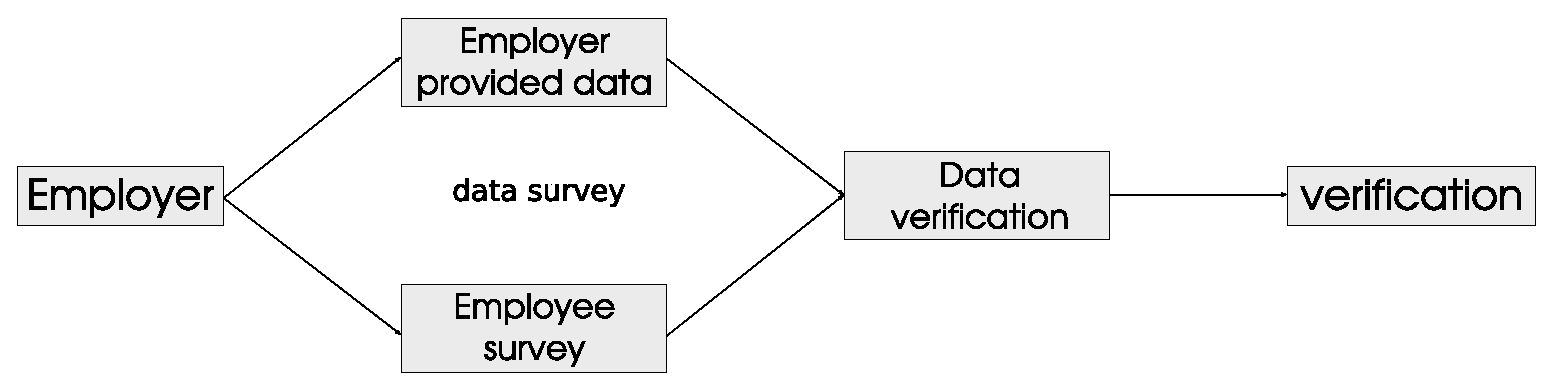
\includegraphics[width=0.9\textwidth]{Bilder/bEquality-project-flow.eps}
	\caption{Project flow graph}
	\label{Project_flow_graph}
\end{figure}
The figure \ref{Project_flow_graph} visualizes the high-level structure of our project.\\
Existing gender-equality indices differ from our project at the points \textit{data survey (employee survey)} and \textit{data} \textit{verification} in the high-level structure and in the final evaulation.\\
We will now explain the high-level structure of our project structure.

\paragraph*{Employer Survey}
There are a few necessary steps for an employer to get a certification.
First, the employer has to to send the data asked for by the given rating framework via a Website. Additionaly the company provides the E-mail-Addresses of their employees. That’s the employer provided data.

\comment{Question: do we really take the e-mail addresses?\\
Or does the employer tells every employee to make an account on our platform and then the employer sends us all generated public keys? (sending of public keys can be done implicitly at the registration of the employee)}

\paragraph*{Employee Survey}
After that, a percentage of employees will be chosen randomly to participate in an employee survey. This survey is used to validate the plausability of the provided data from the employer and to obtain further important private data from employees that cannot be known by the employer.\\

However, this is an easy task for the employee. To set up an account, the employee gets an invitation link from our program and then gets linked to the app, where he/she can set up his/her account. While setting up the account, a public and a private key get generated in the background and linked to the employee account.\\
After the account set-up the company sends all the public-keys generated by the employee account set-up to our framework, this then initiates the survey set-up.\\
When all background work is done, the employee gets a message that the survey is ready. He/she has then just to log into the app, fill out the survey and then submit the data.\\

Everything technical is handled automatically in the background, such that the user just observes a handy interface, and all data is stored on either the blockchain or the IPFS.

\paragraph*{Data Validation}
When all data is gathered from all chosen employees, we split the data into different classes. Either the data from the employees intersect the employer provided data, and is therefore in the \textit{intersecting-data category}, or it is data that is just known or provided by the employee (such as number of sexual harassments or equivalent things).\\

All data from the \textit{intersecting-data category} gets compared by comparing the provided view of the employer and the view of the employee.\\
This comparison then provides a validity factor for the employer provided data.\\

This process of data validation ensures that the data is not corrupted by either humans or bots.\\

\comment{Q: How is validation done exactly?}

\paragraph*{Display Solution/Evaluation}
We would adapt our evaluation to already existing gender-equality indices. But to further improve the evaluation of this evaluation, we would like to evaluate also different indicators for gender-equality and other measures that are important.\\
And because all the data is digitally available, we could also insert classification via artificial intelligence to even further improve the evaluation process.\\
The data evaluation then finally not just results in a single index number, but in a multidimensional spider-diagram, that allows the investor or the company to look closer to existing problems or advantages over the requirement:
\begin{figure}[H]
	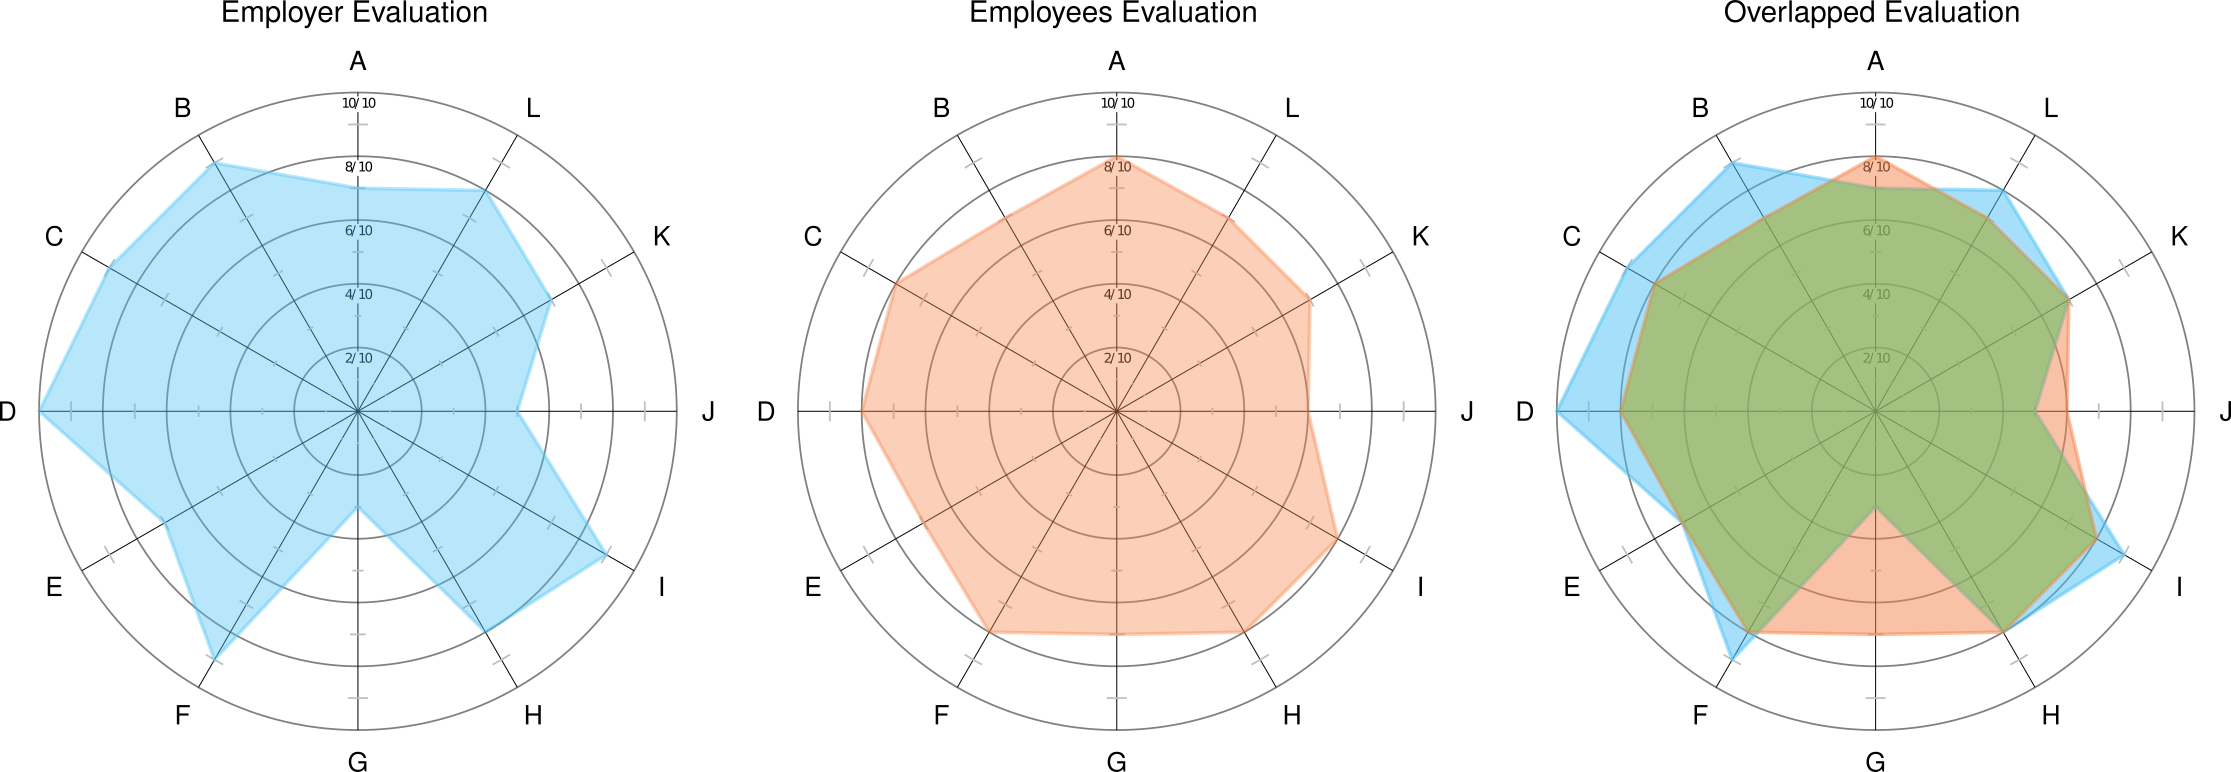
\includegraphics[width=0.95\textwidth]{Bilder/spider-eval}
	\caption{Spider-diagram evaluation example}
	\label{Spider_diagram_evaluation}
\end{figure}
The figure \ref{Spider_diagram_evaluation} provides a flexible evaluation system with detailed feedback.\\
This detailed feedback is useful for company management and also useful for investment decisions by investors that may want to invest in this company. It also implies a feedback system for the company to rate, such that the company knows what to improve in it's employee environment to further imrove it's index.